% !TEX root = ../../../main.tex

\toggletrue{image}
\toggletrue{imagehover}
\chapterimage{logic_gates}
\chapterimagetitle{\uppercase{Logic Gates}}
\chapterimageurl{https://xkcd.com/2497/}
\chapterimagehover{In C, the multiocular O represents the bitwise norxondor gorgonax.}

\chapter{Halbaddierer}
\label{chapter-halbaddierer}

Das Ziel von diesem und den folgenden Kapiteln ist es, ein Schaltnetz zu konstruieren, welches zwei mehrstellige Dualzahlen addieren kann. Die Lernziele für dieses Kapitel lauten:\\

\newcommand{\halbaddiererLernziele}{
\protect\begin{minipage}{\textwidth}
\begin{todolist}
\item Sie definieren, was ein Addiernetz ist.
\item Sie erstellen ein Schaltnetz, welches zwei einstellige Dualzahlen addieren kann.
\item Sie vereinfachen ein Schaltnetz, sodass es weniger Logikgatter benötigt.
\item Sie definieren, was ein Halbaddierer ist.
\end{todolist}
\end{minipage}
}

\lernziel{\autoref{chapter-halbaddierer}, \nameref{chapter-halbaddierer}}{\protect\halbaddiererLernziele}

\halbaddiererLernziele

\section{Addiernetz}

Ein Addiernetz automatisiert die schriftliche Addition von zwei Dualzahlen im Computer.

\begin{definition}[Addiernetz]
Ein Addiernetz ist ein Schaltnetz, welches zwei mehrstellige Dualzahlen addieren kann. Es ist Bestandteil eines Prozessors, eine zentrale Hardwarekomponente des Computers.
\end{definition}

Wir werden das Addiernetz schrittweise über mehrere Kapitel konstruieren. 

\section{Konstruktion des Halbaddierers}

Wir realisieren nun die Addition von \textbf{zwei} Binär\textbf{ziffern} durch ein Schaltnetz. Dies kommt bei der schriftlichen Addition von zwei mehrstelligen Dualzahlen immer in der Spalte ganz rechts vor, wie in folgendem Beispiel zu sehen.

\begin{figure}[htb]
\centering
\begin{equation*}
\begin{tikzpicture}[
    row 3/.style={font=\scriptsize},
    every node/.style={column sep=.5mm, row sep=1mm}]
    \matrix (m) [matrix of math nodes,
        nodes in empty cells,
        %nodes=draw
    ] 
    {
    		& 	& 1 & 0 & 1 & \textbf{1} & [5mm]	\text{1. Summand} \\
	+      & 	&    & 1 & 1 & \textbf{1} &      	\text{2. Summand} \\ 
		& 1 	& 1 & 1 & 1 &    &         	\text{Überträge} \\
        		& 1 	& 0 & 0 & 0 & 0 &      	 \text{Summe} \\                                                  
    };
    \draw[-,color=black, semithick] (m-3-1.south west) -- (m-3-6.south east);
\end{tikzpicture}
\end{equation*}
\end{figure}

Das Schaltnetz muss alle vier Kombinationen von zwei Binärziffern addieren können. Wir fassen die vier Kombinationen in \autoref{table-wahrheitstabelle-halbaddierer} zusammen und verwenden die üblichen Bezeichnungen der Digitaltechnik. Wir können \autoref{table-wahrheitstabelle-halbaddierer} nun als Wahrheitstabelle auffassen und daraus mit den bekannten Tools ein Schaltnetz konstruieren.

\begin{table}[htb]
\centering
\begin{tblr}{|Q[c, m, 2cm]|Q[c, m, 2cm]||Q[c, m, 2cm]|Q[c, m, 2cm]|}
\hline
Bit $x$ & Bit $y$ & Summe $s$ & ausgehender Übertrag $c_{\text{out}}$ \\ \hline[2pt]
0 & 0 & 0 & 0 \\ \hline
0 & 1 & 1 & 0 \\ \hline
1 & 0 & 1 & 0 \\ \hline
1 & 1 & 0 & 1 \\ \hline
\end{tblr}
\caption{Der Übertrag wird ausgehender Übertrag genannt (eng. carry out), da bei der Addition ein Übertrag am Ausgang erzeugt wird.}
\label{table-wahrheitstabelle-halbaddierer}
\end{table}

\subsection{Übungen}

Lösen Sie die Übungen in der vorgegebenen Reihenfolge.

\begin{exercise}
\label{exercise-wahrheitstabelle-halbaddierer}
Erstellen Sie für die Wahrheitstabelle  (siehe \autoref{table-wahrheitstabelle-halbaddierer}) eine Boolesche Formel in \ac{DNF}. Sie müssen also für $s$ und $c_{\text{out}}$ \textbf{jeweils} eine Boolesche Formel in \ac{DNF} erstellen.

\fillwithgrid{2in}
\end{exercise}

\begin{exercise}
Zeichen Sie für die Booleschen Formeln aus \autoref{exercise-wahrheitstabelle-halbaddierer} das dazugehörige Schaltnetz. Es ist \textbf{ein} Schaltnetz mit \textbf{zwei} Eingängen und \textbf{zwei Ausgängen}.

\fillwithgrid{\stretch{1}}

\end{exercise}

\newpage

\section{Der Halbaddierer}

Für die Wahrheitstabelle aus \autoref{table-wahrheitstabelle-halbaddierer} erhalten wir die Formeln $s = (\neg x \wedge y) \vee (x \wedge \neg y)$ und $c_{\text{out}} = x \wedge y$. Damit entsteht das Schaltnetz aus \autoref{half-adder-schaltnetz-1}.

\begin{figure}[ht]
\centering
\begin{circuitikz}
\draw (-2, 1) node[and port] (AND1) {};
\draw (-2, -1) node[and port] (AND2) {}; 
\draw (0, -2.5) node[and port] (AND3) {};

\draw (0,0) node[or port] (OR1) {}; 

\draw (-4,1.5) node[european not port] (NOT1) {};
\draw (-4,-1.5) node[european not port] (NOT2) {};

\draw (OR1.out) node[anchor=west] {$s$};
\draw (AND3.out) node[anchor=west] {$c_{\text{out}}$};

\draw (-8, 0.5) node (x) {$x$};
\draw (-7, 0.5) node[circle, fill, inner sep=1pt] (xC1) {};
\draw (-7, -0.775) node[circle, fill, inner sep=1pt] (xC2) {};

\draw (-8, -0.25) node (y) {$y$};
\draw (-7.5, -0.25) node[circle, fill, inner sep=1pt] (yC1) {};
\draw (-7.5, -1.5) node[circle, fill, inner sep=1pt] (yC2) {};

\draw (AND1.out) |- (OR1.in 1);
\draw (AND2.out) |- (OR1.in 2);

\draw (NOT1.out) |- (AND1.in 1);
\draw (NOT2.out) |- (AND2.in 2);

\draw (x.east) |- (xC1);
\draw (xC1) |- (NOT1.in);
\draw (xC1) |- (AND2.in 1);
\draw (xC2) |- (AND3.in 1);

\draw (y.east) |- (yC1);
\draw (yC1) |- (NOT2.in);
\draw (yC1) |- (AND1.in 2);
\draw (yC2) |- (AND3.in 2);
\end{circuitikz}
\caption{Schaltnetz für $s = (\neg x \wedge y) \vee (x \wedge \neg y)$ und $c_{\text{out}} = x \wedge y$.}
\label{half-adder-schaltnetz-1}
\end{figure}

Das Schaltnetz aus \autoref{half-adder-schaltnetz-1} kann zwei Binärziffern addieren. Es ist somit ein Halbaddierer.

\begin{definition}
Ein Schaltnetz, welches zwei \textbf{einstellige} Dualzahlen (zwei Binärziffern) addieren kann, nennt man \textbf{Halbaddierer} (eng. half adder, kurz \acs{HA}).
\end{definition}

Es gibt verschiedenen Schaltnetze, welche einen Halbaddierer (\ac{HA}) darstellen. Das Schaltnetz aus \autoref{half-adder-schaltnetz-1} ist eine Möglichkeit für die Realisierung. Unabhängig davon, wie wir das Schaltnetz für den Halbaddierer konstruieren, verwenden wir nun die Darstellung aus \autoref{figure-ha-block} für den Halbaddierer. Es repräsentiert ein eigenständiges Bauteil, welches auch so zu kaufen gibt. Wir können es uns so vorstellen, als wäre das Schaltnetz aus \autoref{half-adder-schaltnetz-1} dahinter \say{verborgen}.

\begin{figure}[htb]
\centering
\begin{circuitikz}[american]
	\draw (0,0) node[dipchip, num pins=4, hide numbers, no topmark] (HA) {\acs{HA}};
	\node[left] at (HA.pin 1) {$x$};
	\node[left] at (HA.pin 2) {$y$};
	\node[right] at (HA.pin 3) {$c_{\text{out}}$};
	\node[right] at (HA.pin 4) {$s$};
\end{circuitikz}
\caption{Ein Halbaddierer mit zwei Eingängen ($x$ und $y$) und zwei Ausgängen ($s$ und $c_{\text{out}}$). Die Eingänge repräsentieren zwei einstellige Dualzahlen (zwei Binärziffern). Die Ausgänge zeigen die Summe und den ausgehenden Übertrag (eng. carry out, kurz $c_{\text{out}}$).}
\label{figure-ha-block}
\end{figure}

\begin{figure}[H]
\centering
\begin{minipage}{0.45\textwidth}
\centering
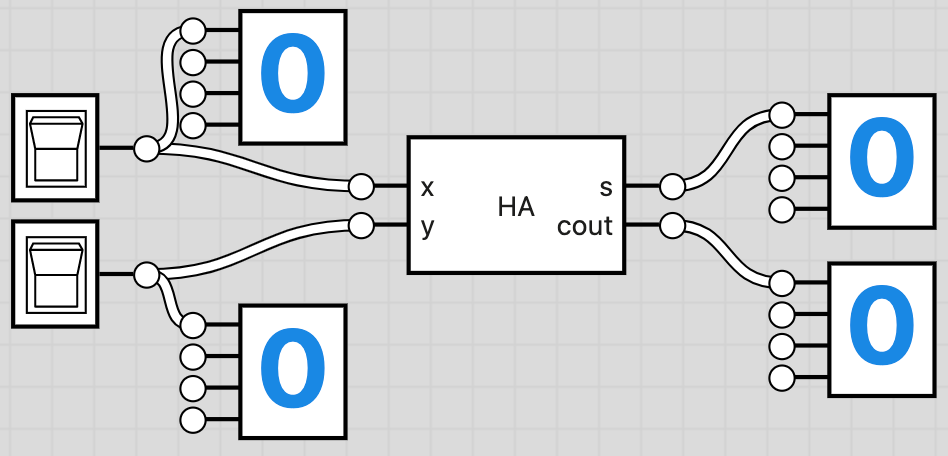
\includegraphics[width=\textwidth]{ha_1}
\end{minipage}
\begin{minipage}{0.45\textwidth}
\centering
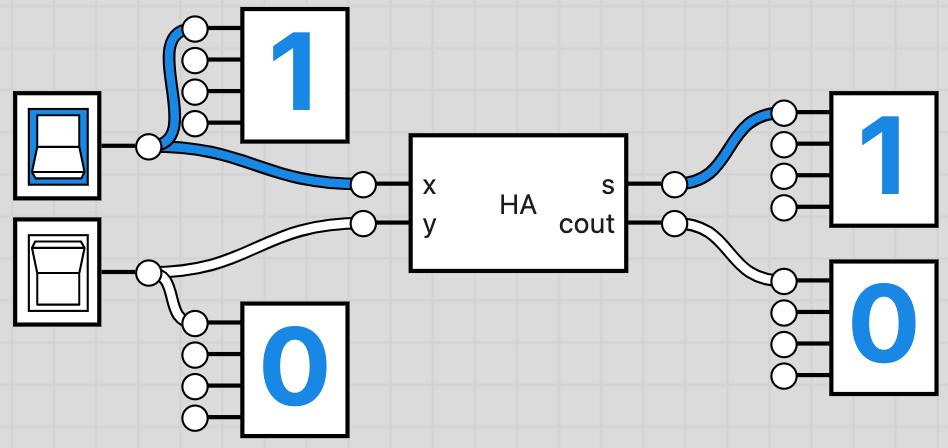
\includegraphics[width=\textwidth]{ha_2}
\end{minipage}
\begin{minipage}{0.45\textwidth}
\centering
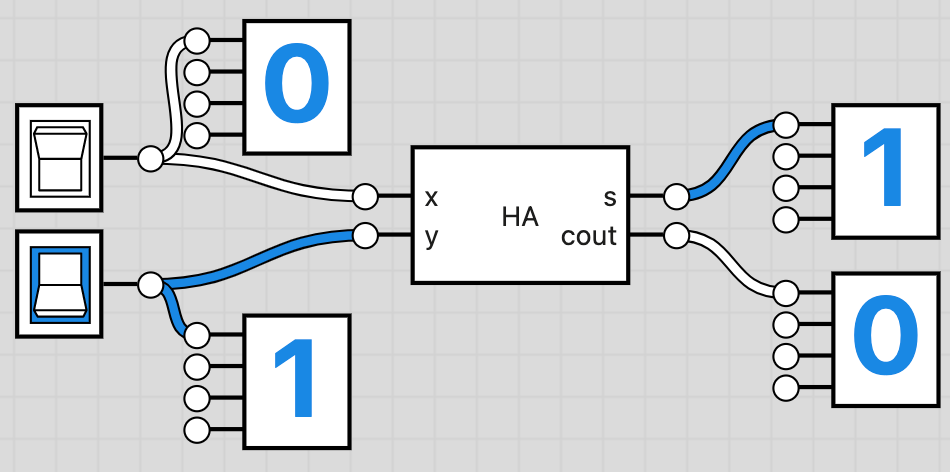
\includegraphics[width=\textwidth]{ha_3}
\end{minipage}
\begin{minipage}{0.45\textwidth}
\centering
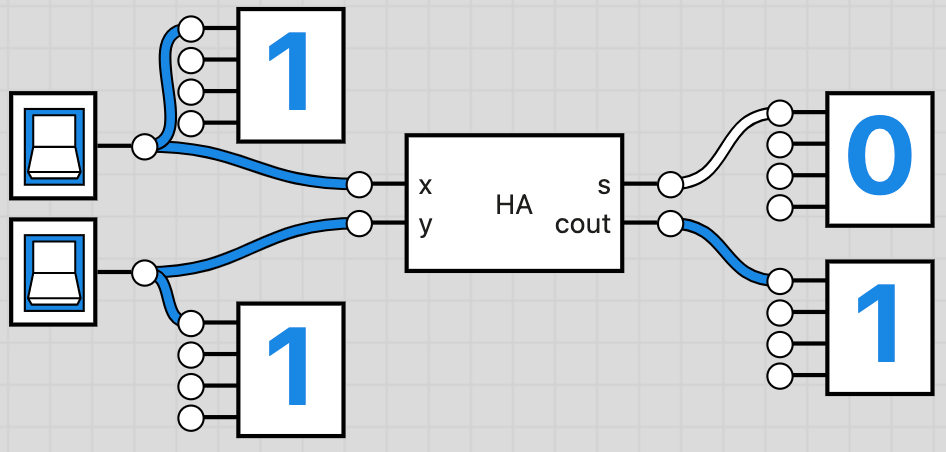
\includegraphics[width=\textwidth]{ha_4}
\end{minipage}
\caption{Der Halbaddierer simuliert in Logicly. Es werden alle vier Kombinationen angezeigt.}
\end{figure}

\newpage

\subsection{Übungen}

Lösen Sie die Übungen in der vorgegebenen Reihenfolge.

\begin{exercise}
Ein Teil des Schaltnetzes für den Halbaddierer lässt sich kompakter darstellen. Vereinfachen Sie die Formel $s = (\neg x \wedge y) \vee (x \wedge \neg y)$, sodass weniger Boolesche Operatoren benutzt werden. Schauen Sie sich dazu gegebenenfalls nochmals Übung \ref{exercise-xor-nor-nand-xnor} an.
\fillwithgrid{1in}
\end{exercise}

\begin{exercise}
Zeichnen Sie erneut das Schaltnetz für einen Halbaddierer. Berücksichtigen Sie dieses Mal Ihre Ergebnisse aus der vorherigen Aufgabe.
\fillwithgrid{\stretch{1}}
\end{exercise}